\chapterp{3p}{Current online SWR detection}\label{ch:BPF}

This chapter discusses the current state-of-the-art method in online SWR detection. This method is very similar to the procedure for offline ripple detection described in \cref{ch:offline}: we also select a single recording channel containing ripples, band-pass filter its data through the ripple band, and apply a detection threshold to the envelope of the filter output.
% todo: multi-channel (Dutta, Ciliberti)

The difference is that the SWR detection must now happen under real-time constraints. No future samples can be used when deciding whether the current recording sample belongs to an SWR event. This means that the used band-pass filter (and in some studies, also the envelope estimation method) must necessarily introduce latency.



\section{Online band-pass filters}

% continue: summary of lit quotes on filter types.



\section{Online envelope estimation}

The real-time constraint also means that we can no longer use the Hilbert transform to calculate the envelope $n_t$ of the band-pass filter output $o_t$. In practice, the band-pass filter output is often simply rectified (i.e. $n_t = \abs{o_t}$).
% Although the resulting jagged signal is not as visually pleasing as the Hilbert-transform based envelope, it is effective for signal detection.
% (In \citefull{Sethi2014}, it was shown that more advanced online envelope estimators do not yield better detection performance).

Extensions of simple rectification have also been used. In \citefull{Jadhav2012}, the online envelope $n_t$ is an exponentially weighted moving average (EWMA) of $\abs{o_t}$. They use a slightly higher weight for $\abs{o_t}$  whenever $n_t < \abs{o_t}$ (see \cref{apx:online-SWR-detection-literature}. In \citefull{Dutta2018}, $\abs{o_t}$ is smoothed with a 50 Hz low-pass FIR filter.

Both methods add latency. The EWMA method of \citeauthor*{Jadhav2012} delayed the envelope by about 2 milliseconds when applied to our recording. The FIR low-pass filter of \citeauthor*{Dutta2018} has a constant group delay of about 5 milliseconds.

Smoothing $\abs{o_t}$ yields a visually more pleasing envelope. This is not a requirement for online SWR detectors however. Because smoothing adds latency, we do not smooth our online envelope $n_t = \abs{o_t}$.




% task: what's used in online SWR-detection literature.

% task: for each filter, a separate plot (in appendix) of its parameter range (rp, rs, width). DONE
% task: a plot of groupdelay in ripple band, and ratio of sumated magnitude responses passband versus stopband. DONE

% task: write about difference in fs (and therefore normalized frequencies & numtaps)

% Goal of this chapter:
%  - Establish baseline, implement SOTA
%  - Find best digital online BPF.

% Idea: implement Ego-Stengel (cont2discrete(butter)), Jadhav (best IIR), Talakoub / Dutta (FIR). With simple abs.
% OR: find equivalent of these in your already existing graphs. Annotate them (with thick dot and arrow).
%   Decision here: each study has different band.
%   (100-400, 100-400, 80-150, 150-250).
%   Let's plot both.


\clearpage
\begin{figure}
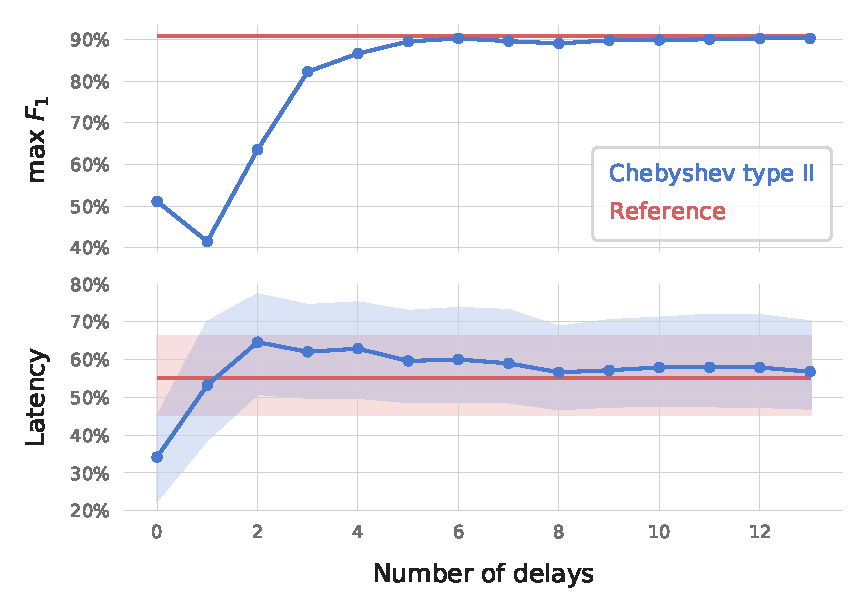
\includegraphics{figures/searcharray-cheby2}
\captionn[, ]{Performance of Chebyshev type 2 IIR-filters}{for different filter orders. The minimum stop-band attenuation was set to 40 dB.}
\end{figure}

\begin{figure}
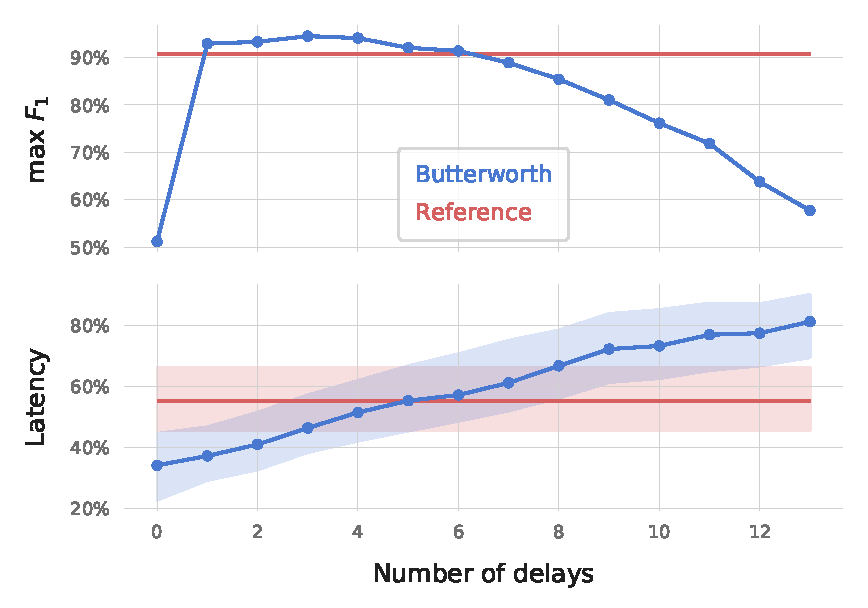
\includegraphics{figures/searcharray-butter}
\captionn[, ]{Performance of Butterworth IIR-filters}{for different filter orders.}
\end{figure}
